\documentclass[a4paper,oneside,twocolumn]{article}
\usepackage{graphicx,islab-resume,boxedminipage,fancyvrb,amsmath,amssymb,amsfonts}
\usepackage{cases}
\usepackage{listings}
\usepackage{ascmac}
\usepackage{framed}
\usepackage{amsmath}
\usepackage{tikz}
\usepackage{algorithm}
\usepackage{algorithmic}
\usepackage{float}
\usepackage{caption}

\author{MOLINA TORO David}
\seminar{2026 Spring Semester Integrated System Design Seminar}
\date{2026-06-26}
\title{Design of a Rotational Floating Self-Excited TENG}
\totalpage{1}
\begin{document}
\maketitle

\section{Abstract}

The search for alternative energy sources is a high-priority objective in today's society. Significant reductions in power consumption and physical size for microcontroller-based systems, combined with new long-range communication technologies, enable the deployment of sensors in remote locations via mesh networks, thereby allowing for the affordable implementation of decentralized systems \cite{FISCHER2012}. This research aims to analyze recent advances in this field and to identify viable alternatives for addressing these types of challenges.


\section{Introduction}

Triboelectric nanogenerators (TENGs) show promise as a renewable energy source capable of powering low-consumption autonomous systems. They operate by harnessing the triboelectric effect, in which electrostatic charges are transferred between materials with differing properties when friction occurs between them. Most examples focus on compression-expansion systems or sliding rotational motion, although other designs utilize friction with elements such as water \cite{LIN2013}.

However, harvesting energy using these devices is challenging. The movement of the electrodes and the dielectric causes the generator's impedance to change continuously throughout each cycle. This leads to issues regarding proper impedance matching between the source and the load. Identifying a system capable of operating under these conditions, while delivering stable power and ensuring component durability, is crucial for their deployment in remote environments where other energy sources are impractical.

This research focuses on sliding-mode TENGs, specifically those based on the circular motion of contacting materials, which appear to offer a favorable balance between efficiency and durability.

\subsection{Sliding TENG}

Sliding-mode TENGs (S-TENGs) have been considered among the most significant since their emergence \cite{NIU2015}. This type of generator employs a pair of triboelectric surfaces that slide against each other involving contact or lateral friction, diagram of operation shown in Figure \ref{fig:SlidingTENG}. They offer high output compared to other types, making them ideal for continuous energy harvesting. However, they are subject to wear caused by friction between the surfaces, and the high voltage peaks generated between them can lead to air breakdown, completely nullifying the triboelectric effect.

\begin{figure} [H]
  \centering
  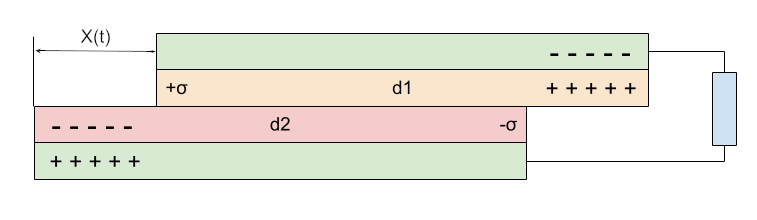
\includegraphics[width=0.95\columnwidth]{Images/Sliding TENG.png}
  \caption{Diagram showing the principle of operation for an S-TENG}
  \label{fig:SlidingTENG}
\end{figure}

\subsection{Floating TENG}

Unlike S-TENGs, floating TENGs (F-TENGs) do not generate energy through direct friction between their contacts; instead, an electrode floats and operates in a non-contact sliding mode, diagram of operation shown in Figure \ref{fig:FloatingTENG}. Consequently, the device undergoes negligible wear during operation and maintains high power output due to minimal frictional losses in the system. However, the output can be severely reduced if the existing charge on the contacts drops abruptly.

\begin{figure} [H]
  \centering
  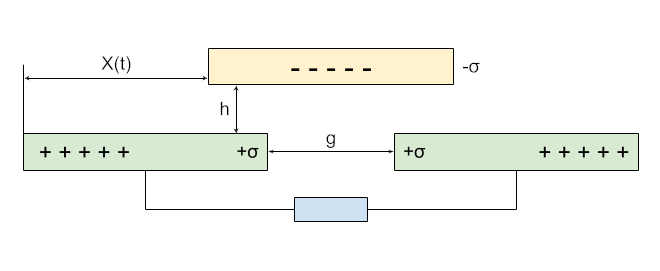
\includegraphics[width=0.95\columnwidth]{Images/Floating TENG.png}
  \caption{Diagram showing the principle of operation for an F-TENG}
  \label{fig:FloatingTENG}
\end{figure}

\subsection{FSS-TENG}

Floating self-excited charge TENGs (FSS-TENGs) go a step beyond F-TENGs by incorporating charge feedback to one of the contact pairs. They maintain high durability due to their floating-mode operation and increase efficiency thanks to the charge feedback. On the other hand, they are more complex than their counterparts, as they require external circuits such as a Bennet or Villard multiplier. Nevertheless, their efficiency remains high across a wider range of angular velocities, and contact wear is minimal, just as with F-TENGs.

\vspace{0.5cm}


\section{Related Research}

Recent research on circular-motion-based TENGs highlights two complementary approaches to enhancing performance: amplifying surface charge density via excitation circuits and reducing friction between surfaces through non-contact operating modes.

Bipolar charge injection, achieved using a voltage multiplier circuit (VMC) connected to the two electrode groups on one of the surfaces, significantly increases the potential difference and, consequently, the amount of charge transferred between the contacts \cite{XIA2025}. Tests show that charge transfer increases by approximately two orders of magnitude compared to a system without excitation, while maintaining non-contact operation and high durability. Example shown in Figure \ref{fig:InjectionTENG}.

\begin{figure} [H]
  \centering
  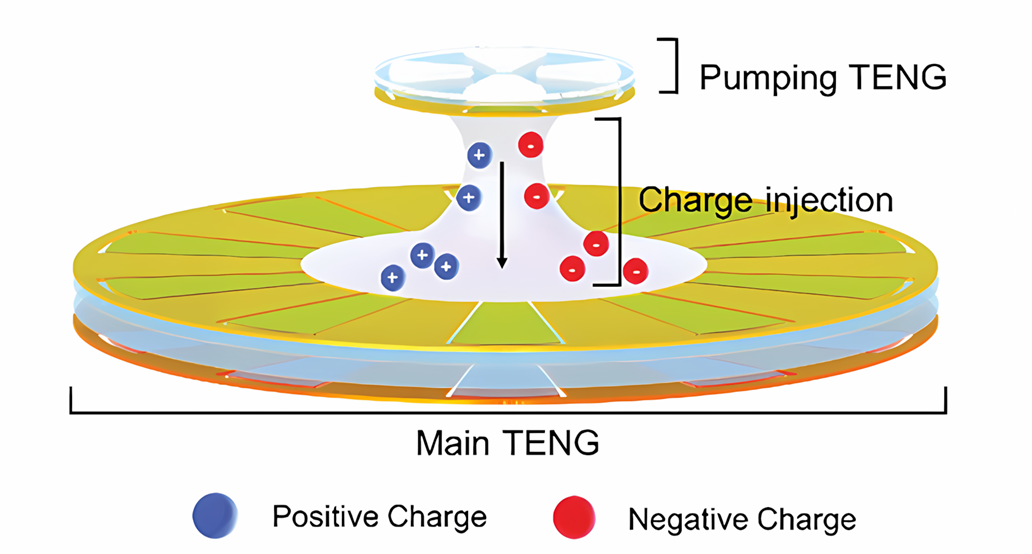
\includegraphics[width=0.95\columnwidth]{Images/Injection TENG.png}
  \caption{Diagram of an FSS-TENG with a charge injection mechanism \cite{SHAOBO2023}}
  \label{fig:InjectionTENG}
\end{figure}

In parallel, other models incorporate a secondary generation unit that injects charge into the main TENG. This secondary unit relies on gentle contact friction, utilizing polyester brushes against copper contacts \cite{SHAOBO2023}. Charge injection via this system achieves very high densities, up to 74.62 µC/cm², while maintaining an output power close to the initial level after 1,000,000 operating cycles.

Finally, optimizing contact surface geometries plays a key role in enhancing the performance of this type of TENG. The effectiveness of optimization techniques using Gaussian Process Regression is demonstrated by their application in defining Bezier curves that increase average power output by up to six times compared to a traditional design \cite{YOON2025}. Selectively reducing the overlap area based on the rotation angle increases charge density in the active region without increasing capacitance losses.

All three studies demonstrate how incorporating charge injection, via VMC or secondary generators, and optimizing geometric design make it possible to overcome the limitations of traditional designs. For rotational FSS-TENG designs, bipolar injection and coplanar pumps offer practical alternatives for increasing open-circuit voltage (Voc) and short-circuit charge transfer (Qsc) without compromising generator durability. However, these approaches require careful design, as controlling the stator-rotor gap and managing electrostatic coupling effects are essential to avoid unwanted attraction between the contacts.


\section{Design}

This research involved multiple tasks related to the design, implementation, and initial validation of a rotational FSS-TENG system. These stages focused on three main processes: developing a controller for a stepper motor to manage the FSS-TENG's movement; designing the stator and rotor geometries and fabricating them using PCB technology; and constructing a test bench to conduct an initial experimental evaluation of the prototype.

\subsection{TENG Structure}

First, the design of the FSS-TENG stator and rotor was developed, based on optimization criteria reviewed during the research phase. Specifically, the geometry of the contact leading edges was improved to enhance the performance of non-contact, sliding-mode rotary TENGs. Parameters such as the number of contacts, the gap between the stator and rotor, the total surface diameter, and the rotor's angular velocity were taken into account. Additionally, a connection architecture was established to enable the future implementation of charge injection strategies and contact group modifications. The final design was implemented on a pair of PCBs with a diameter of 200 mm, featuring a total of 20 contacts per surface.

\subsection{Motor Driver}

Secondly, a control system was developed for the Nema17 stepper motor responsible for providing the rotational movement to the FSS-TENG rotor during testing. The initial version of the controller was implemented using a driver based on the A4988 chip paired with an RP2040 microcontroller, resulting in a very low-cost system that included a user interface via an OLED display and a rotary encoder. However, initial tests revealed several design limitations, including abrupt speed fluctuations and missed steps during operation at speeds exceeding 3 Hz.

Consequently, a second version of the controller was designed using the TMC2209 chip, a component found in many commercial devices that offers features capable of resolving the previous issues. This new design was implemented on a fully custom PCB incorporating an ESP32-S3-based development board, thereby providing the system with wireless connectivity. To simplify the user interface, the rotary encoder was replaced with a series of board-mounted buttons, allowing for interaction with the controller without the need for a computer or additional device. A view of the final motor driver can be seen in Figure \ref{fig:StepperDriver}.

\begin{figure} [H]
  \centering
  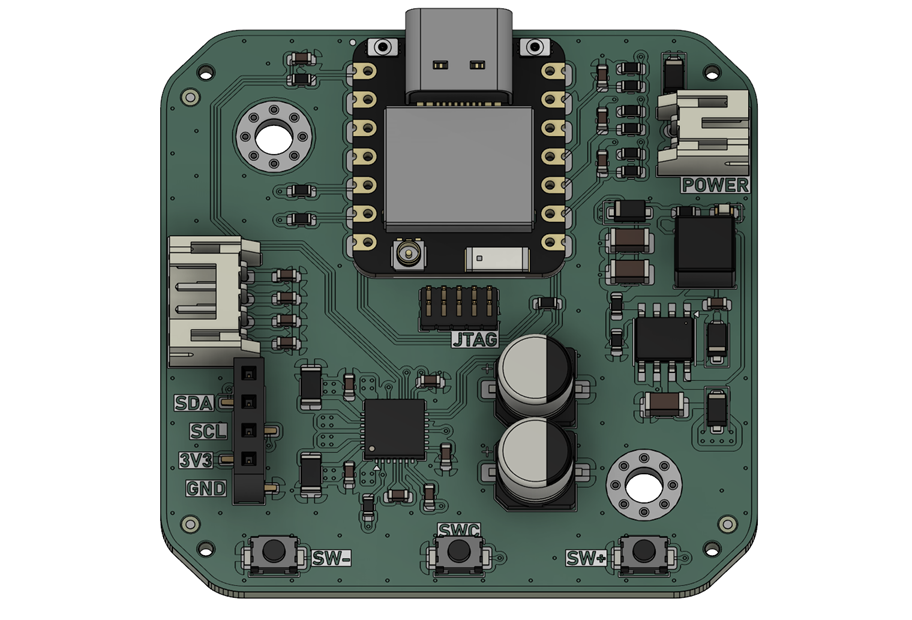
\includegraphics[width=0.95\columnwidth]{Images/Stepper Driver.png}
  \caption{Model view of the designed stepper motor driver PCB}
  \label{fig:StepperDriver}
\end{figure}

\subsection{Test Bench}

Finally, a PLA-printed test rig was developed in which the generator's rotational movement occurs in the horizontal plane, shon in Figure \ref{fig:TestBench}. This rig allowed for the integration of the stepper motor, the motor control board, the TENG's mechanical supports, and a spacer, to ensure separation between the rotor and stator, onto a single platform. However, initial tests revealed the system's limitations; a lack of fine control over orientation and contact spacing, combined with excessive friction between the two discs, severely hindered the generator's smooth operation. Thanks to the capabilities of the controller used, initial validation was possible, albeit at the cost of high-power consumption to enable the motor to drive the platform's movement.

\begin{figure} [H]
  \centering
  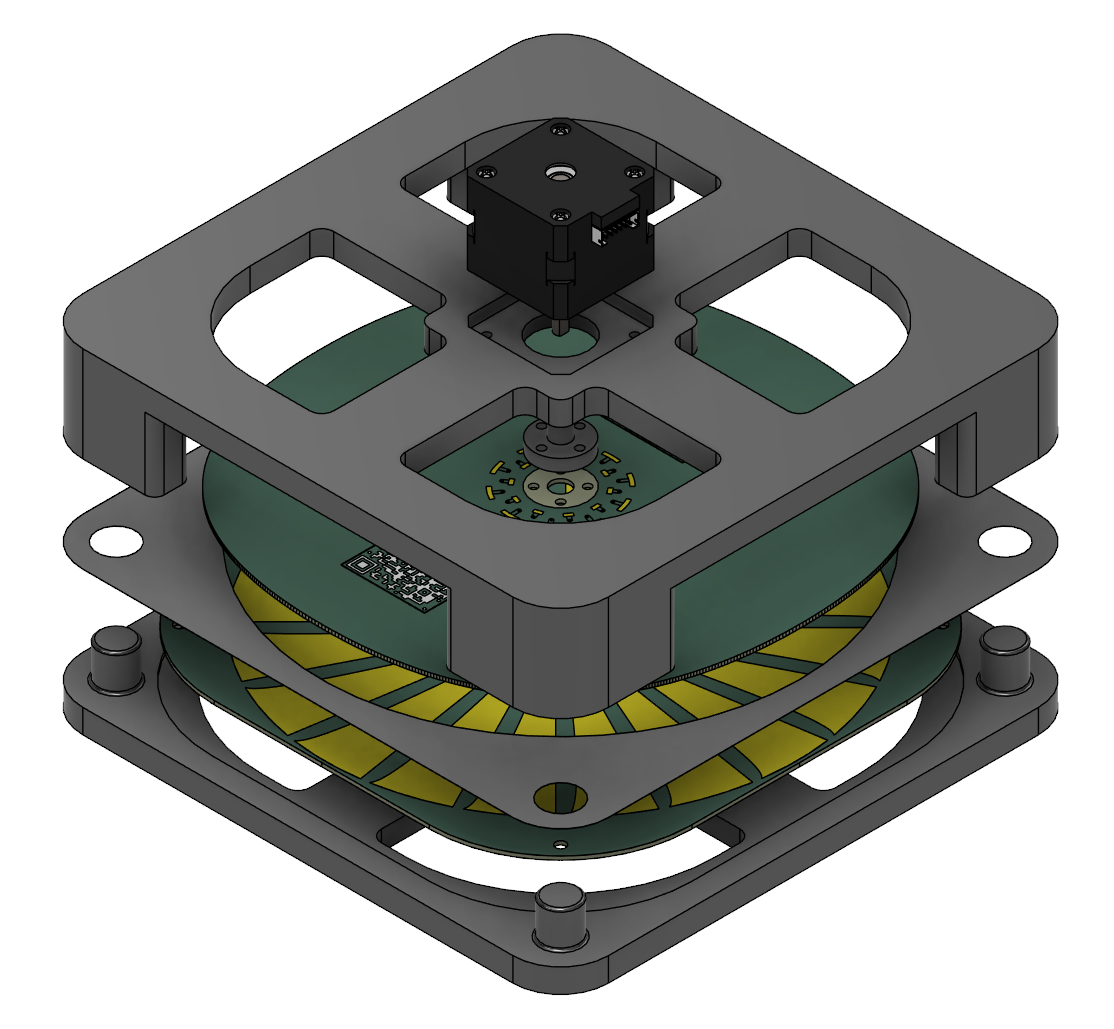
\includegraphics[width=0.95\columnwidth]{Images/Test Bench.png}
  \caption{Model view of the designed test bench prototype}
  \label{fig:TestBench}
\end{figure}

Overall, this work establishes a solid foundation for the subsequent stages of system optimization, addressing mechanical, electrical, and geometric aspects.


\section{Results}

Initial simulations in the LTspice environment made it possible to verify the general behavior of the FSS-TENG model (shon in Figure \ref{fig:LTSpiceFSSTENG}) under various operating conditions. In particular, it was observed that generator performance improves significantly when the gap between contacts is reduced (Figure \ref{fig:SimulationGap}) and the rotation speed is increased (Figure \ref{fig:SimulationRPM}). In practice, however, there are limitations; depending on the implementation environment, it may not be feasible to achieve very high angular speeds while reliably maintaining the contact gap.

% \begin{figure} [H]
%   \centering
%   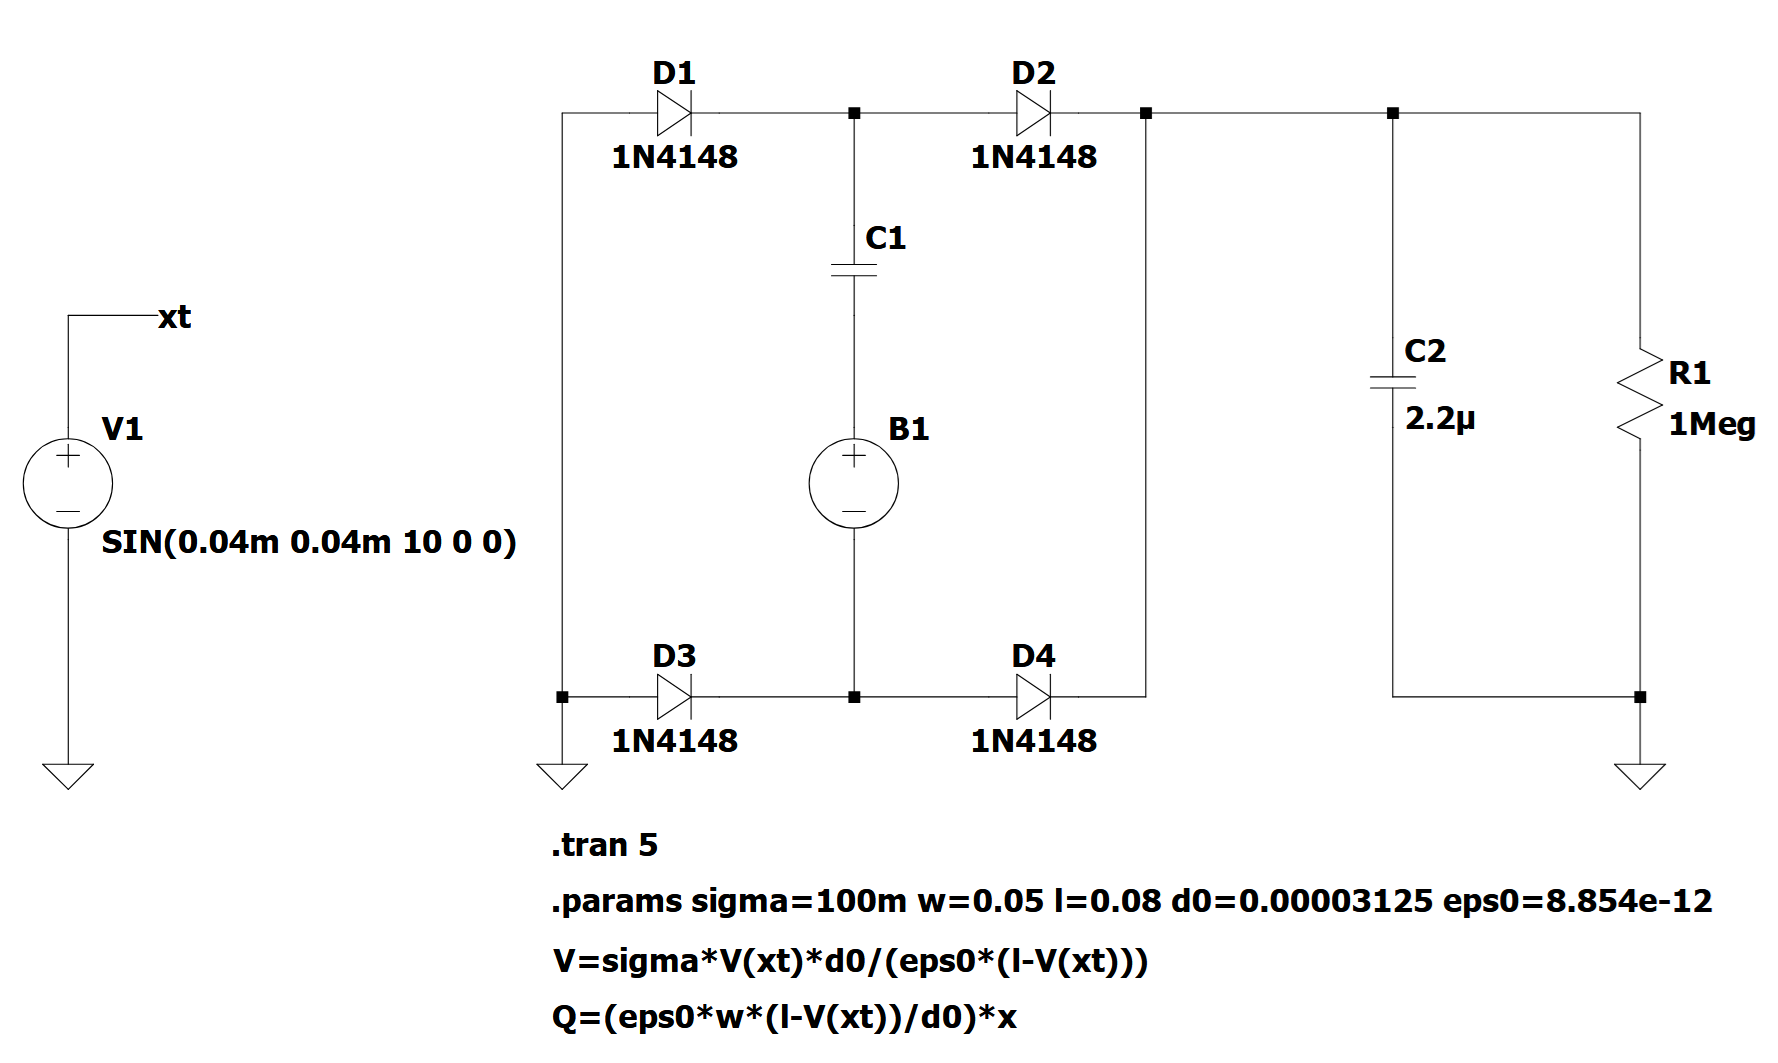
\includegraphics[width=0.95\columnwidth]{Images/LTSpice FSS TENG.png}
%   \caption{Simulation circuit for the FSS-TENG in LTspice}
%   \label{fig:LTSpiceFSSTENG}
% \end{figure}

\begin{figure} [H]
  \centering
  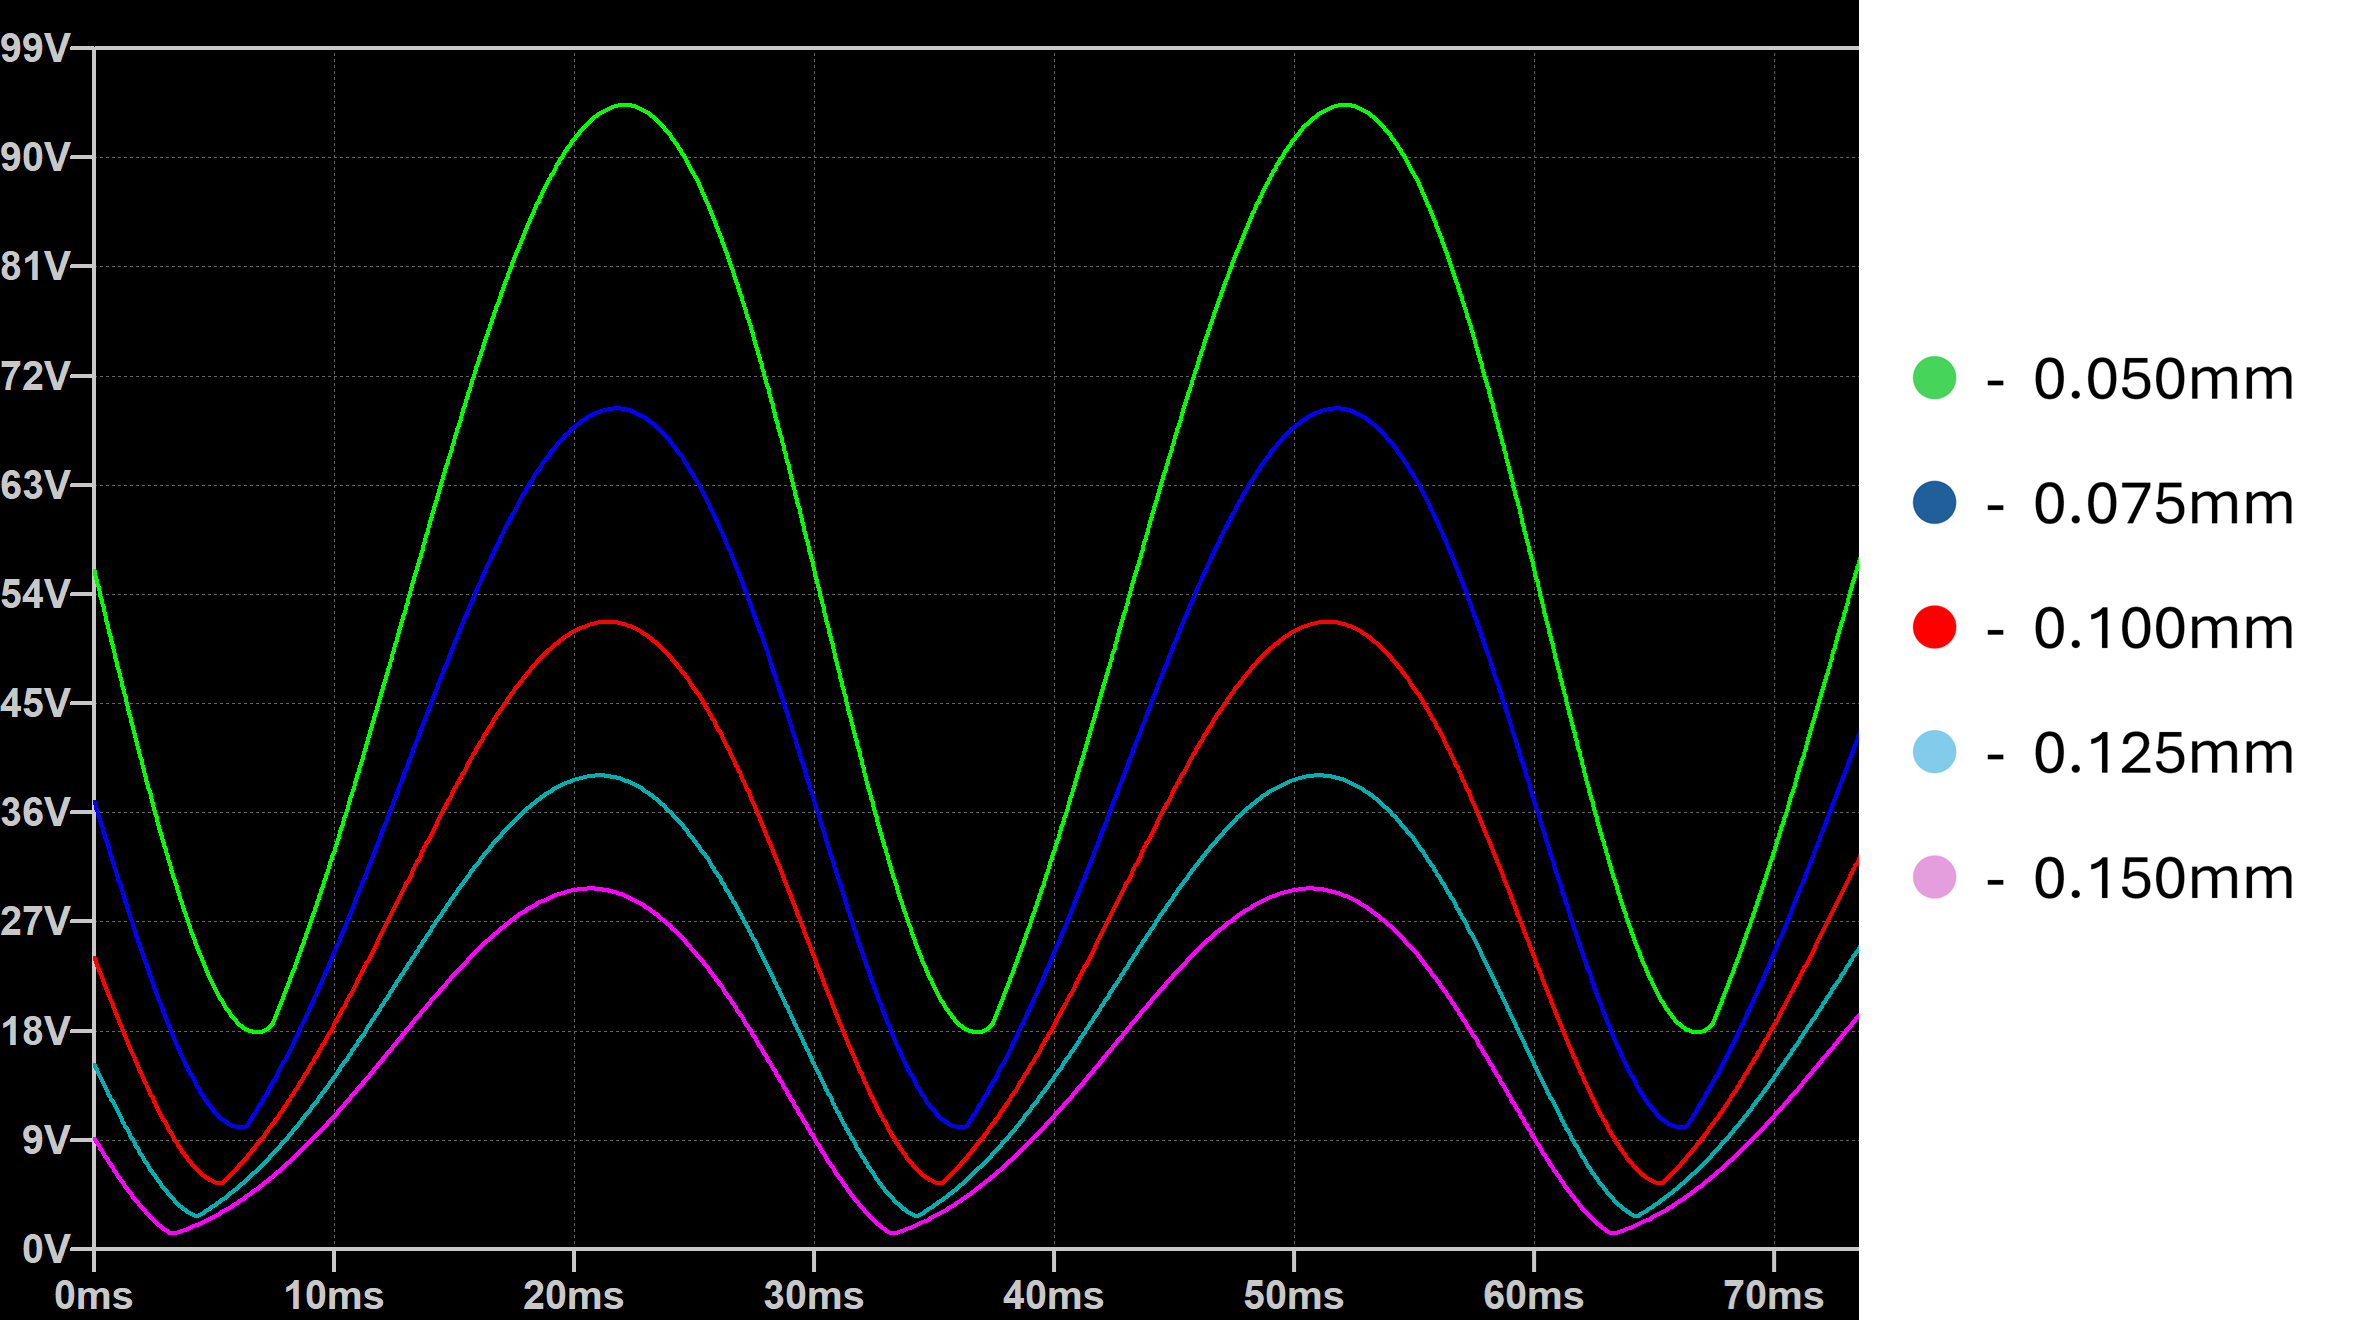
\includegraphics[width=0.95\columnwidth]{Images/Simulation Gap.png}
  \caption{Open-circuit voltage at different air gap between contacts}
  \label{fig:SimulationGap}
\end{figure}

On the other hand, increasing the number of contacts raises the generation frequency while reducing the effective area available for charge transfer. Consistent with previous research, the simulation revealed a clear relationship between output power and load resistance, demonstrating that the system has an optimal operating range where charge transfer is maximized.

\begin{figure} [H]
  \centering
  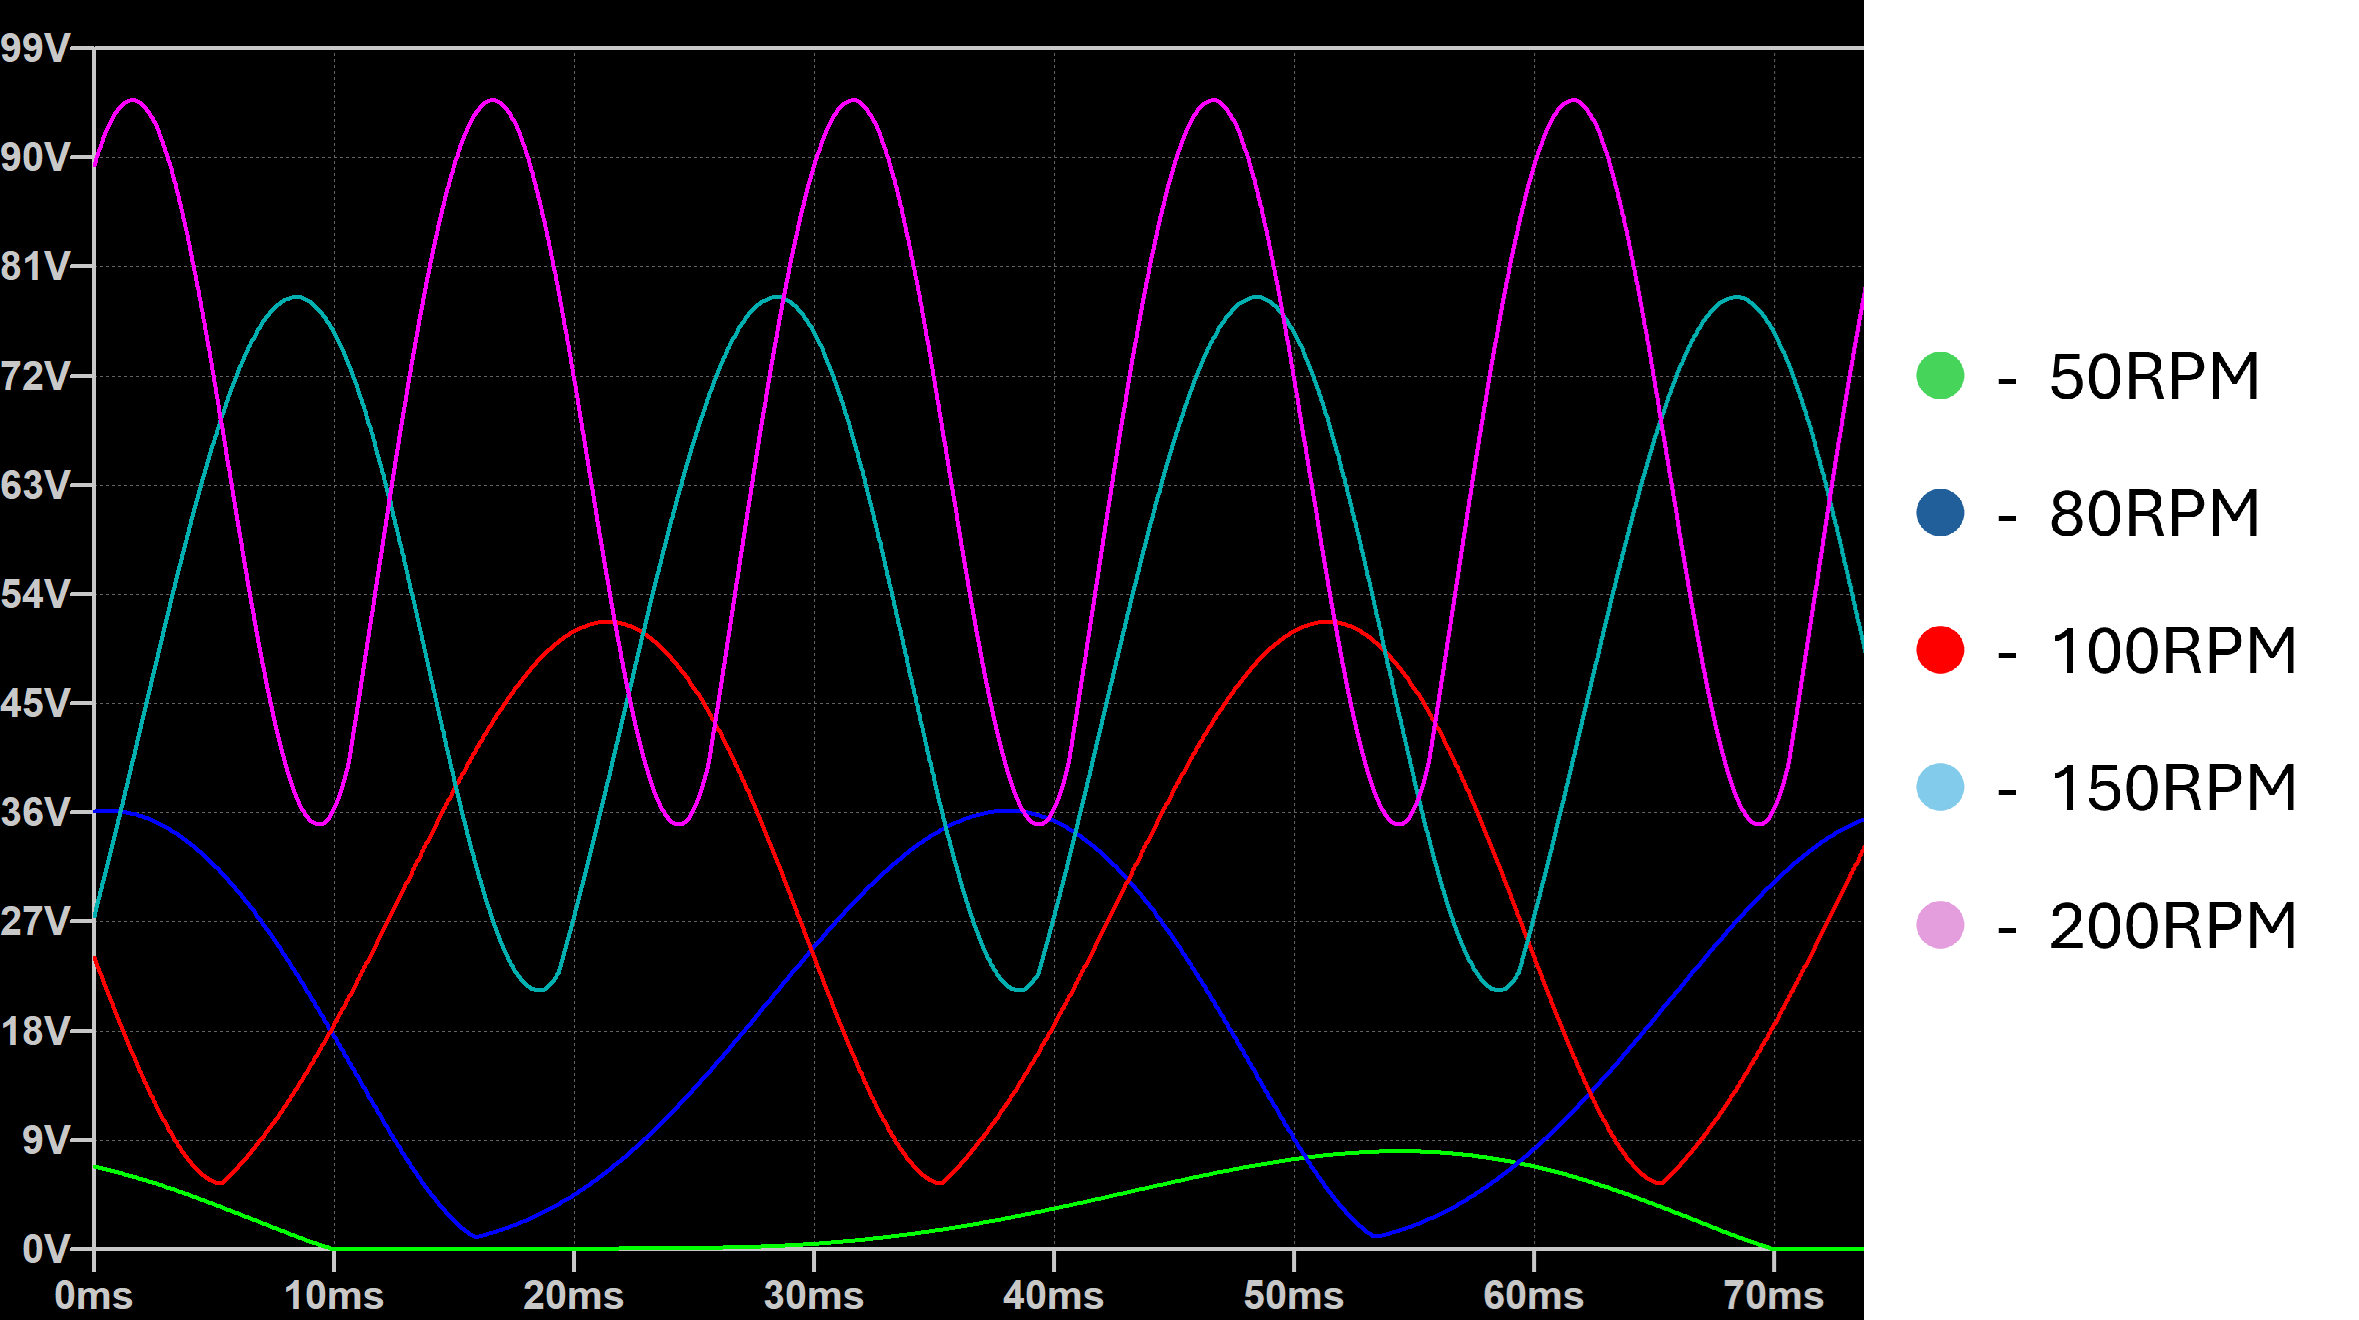
\includegraphics[width=0.95\columnwidth]{Images/Simulation RPM.png}
  \caption{Open-circuit voltage at different rotational speeds}
  \label{fig:SimulationRPM}
\end{figure}

Initial experimental tests of the FSS-TENG demonstrated the prototype's capabilities. These tests involved measuring the FSS-TENG's open-circuit output voltage, without external charge injection, using the oscilloscope probe's own 1 M resistance as the load. The results obtained are shown in \ref{tab:TestResults}.

\begin{table}[H]
  \centering
  \begin{tabular}{|p{1.5cm}|p{2.5cm}|p{2.0cm}|}
  \hline
  \textbf{Speed (rpm)} & \textbf{Voltage pk-pk (V)} & \textbf{Frequency (Hz)} \\
  \hline
     30 & 11.4 & 26.3 \\[0.1cm] \hline
     100 & 14.5 & 36.9 \\[0.1cm] \hline
     200 & 21.9 & 65.7 \\[0.1cm] \hline
     300 & 32.6 & 99.3 \\[0.1cm]
  \hline
  \end{tabular}
  \caption{Open-circuit output voltage for the FSS-TENG prototype} 
  \label{tab:TestResults}
\end{table}


\section{Future Work}

For future work, the primary objective will be to improve the design of the test rig used to evaluate the FSS-TENG model. A key requirement is to maintain the gap between the stator and rotor with high precision while allowing for adjustments based on specific needs. In this type of TENG, the distance between the contacts directly influences electrostatic coupling and effective capacitance. Consequently, constructing a rigid structure, combined with a fine-adjustment alignment mechanism, is crucial for analyzing the generator's behavior.

Furthermore, incorporating a charge injection system is essential for this type of non-contact sliding-based system. Recent studies have shown that the simultaneous injection of positive and negative charges increases the potential difference between the generator contacts, thereby enhancing charge extraction. For an FSS-TENG, this strategy significantly improves performance without compromising the qualities that ensure high durability.

Finally, development will proceed with the integration of an electronic stage dedicated to conditioning the FSS-TENG output to enhance the system's overall efficiency. In this context, the Dual-Output Rectifier (DOR, shown in Figure \ref{fig:DualOutput}) offers a particularly promising approach, as it rectifies the generator's output and distributes it both for useful power generation and to a control stage for a switching circuit based on a flyback converter \cite{SHI2024}. Experimental results indicate that this architecture achieves a two- to threefold increase in peak power compared to a conventional full-wave rectifier operating at frequencies of 2 and 3 Hz. Taken together, refining the test bench design, incorporating a charge injection system, and integrating electronics to optimize performance constitute a viable path for enhancing the capabilities of the proposed system.

\begin{figure} [H]
  \centering
  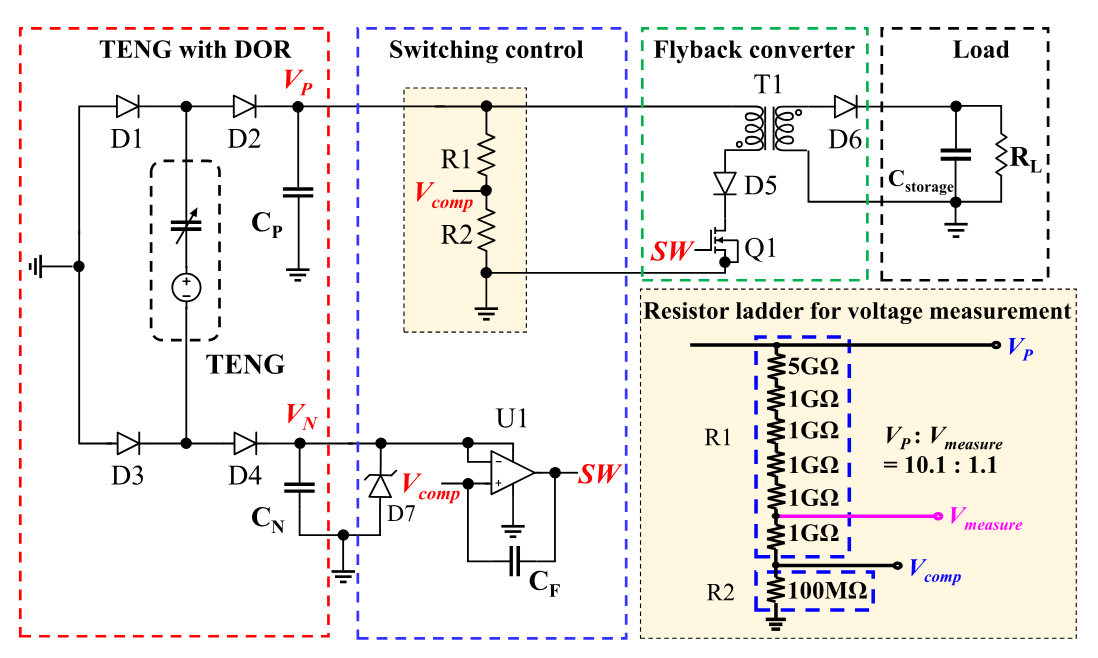
\includegraphics[width=0.95\columnwidth]{Images/Dual Output.png}
  \caption{Diagram of application for the Dual-Output Rectifier circuit \cite{SHI2024}}
  \label{fig:DualOutput}
\end{figure}

\vspace{0.5cm}
\bibliography{ref}
\bibliographystyle{IEEEtran}
\end{document}
